\chapter{Introduction}

\label{chapter:intro}

Micro unmanned aerial vehicles (MAVs, also called drones or unmanned aerial vehicles, UAVs) recently saw a rise in usage across various fields. 
Drones are already widely used in cinematography \cite{Mademlis2020}, advertising \cite{Ullah2021} and agriculture \cite{Kim2019}. 
City emergency departments also use MAVs - firefighters can see and evaluate the situation from the sky, localize the source of fire and put it out \cite{Pritzl2021}.
Another field where MAVs can be used in nearest future is transportation. 
Fast parcel delivery \cite{She2021} and content transportastions \cite{Gupta2021,Aloqaily2022} are quite promissing fields of UAV application together with smart city concepts evolving \cite{Ortiz2019}.
Nowadays, even collaborative transportation systems are becoming realistic - multi-robot swarming algorithms are better developed, and that allows their usage for the transportation of large objects \cite{Bacelar2020} that one drone can not lift. 
MAVs are also widely used in the military industry.

As drones are used so widely, there is a large demand for an increase in drone-related safety. 
Many commercially available drones are expensive and quite heavy, so accidents can be costly and dangerous to property and human health. 
Even if a drone is on a remote control, obstacles can be hard to spot and avoid when the pilot flies a long distance.
Same about flying in a forest or in cities (in situations when it is legal, for example - emergency departments and moviemakers can do it), sometimes obstacles can not be observed.
In such situations, the best for the pilot would be to use a first-person view glasses, which provide a field of view (FOV) not bigger than the FOV of a human's eyes (which is about $130^\circ$), but dangerous obstacles can appear from any side.
In this sense, autonomous robots can see and avoid obstacles much better, but only if they have a well-designed system running onboard and enough sensors to cover the area around a drone.

Automatic obstacle avoidance systems become especially important in closed environments with many obstacles, such as a forest, a city, or indoor environments.
To ensure complete coverage of the surroundings of the MAV for the collision avoidance system, it can be equipped with multiple sensors pointing in all directions.

Considering this context above, a compact obstacle avoidance system is a perspective field for research. 
Even though the idea is not new, there is no complete visual obstacle avoidance system for MAVs that can cover all space around them with a small amount of sensors.
The best, for now, can be the Skydio system\footnote{\href{https://www.skydio.com/skydio-autonomy}{Skydio autonomy: https://www.skydio.com/skydio-autonomy }} which has six 4k $200^\circ$ navigation cameras, and Neural Networks for the environmental analysis, obstacle avoidance and path planning \cite{Skydio}. 
It is available only for US militaries.
The DJI Mavic 3 drone\footnote{\href{https://www.dji.com/cz/mavic-3}{DJI Mavic 3: https://www.dji.com/cz/mavic-3}} seems to be a better solution with eight cameras and an infrared sensor at the bottom. 
Mavic's cameras have almost no overlapping fields of view, so probably they also use some Neural Networks for their obstacle avoidance system. 

Unfortunately, they have no publications, system specifications or implementation details, so it is only a conclusion from publicly available information.

\begin{figure}[t]
    \centering
    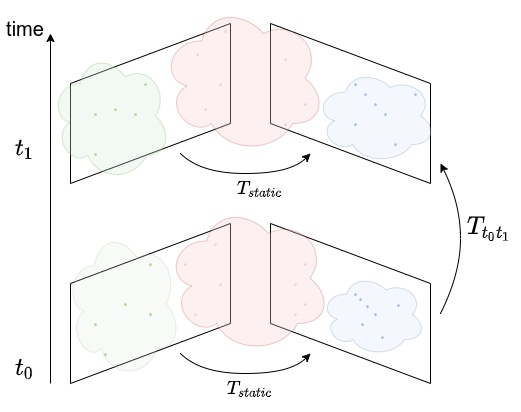
\includegraphics[width=0.6\textwidth]{graphics/general_scheme.png}
    \caption{ A general scheme of the multi-camera obstacle detection problem.}
    \label{fig:intro_general}
\end{figure}

\autoref{fig:intro_general} presents a scheme of the proposed system.
In the figure, $T_{static}$ is the transformation between two cameras onboard the MAV obtained with stereo pair calibration. 
At the time $t_0$, a new pair of images is captured by the cameras.
A feature detector extracts points of interest from the image.
Points that lie in the part of the images corresponding to a section of the cameras' field of view that overlaps (the red point cloud in \autoref{fig:intro_general}) are then selected, and correspondence matches between these points from the two images are found based on their features.
A calibrated projection model of the cameras and the transformation $T_{static}$ are used to estimate 3D points from the matched point pairs.
Then at time $t_1$, when a new pair of images is received, the same process is repeated. 
In parallel, an incremental Structure from Motion (SfM) algorithm processes sequences of images from each camera separately to estimate 3D points corresponding to nearby objects in the environment. However, monocular SfM algorithms can generally only estimate the environment up to an unknown scaling factor \cite{SfM}. To address this problem, the red point cloud is used to find the scale of the points obtained using the SfM algorithm from images captured at $t_0$ and $t_1$ (the blue and green point clouds in \autoref{fig:intro_general}).

\section{Related Works}

There are many approaches to tackling MAV obstacle avoidance in the published literature using various sensors.
In most articles, a stereo pair of two parallel cameras looking in the same direction (classical stereo pair) \cite{Lin2021,Ruf2018,Oleinikova2015,Back2020} are used for that, but there are also, monocular vision approaches \cite{Mejias2010,Zhang2019,Bills2011}, Light Detection and Ranging (LiDAR) (2D or 3D) \cite{Ramasamy2016}.
Sonars (ultrasonic) and time of flight sensors have low accuracy and are sensitive to noise, and they are not used alone but in combinations with others \cite{Gageik2015,Nor2017}. 
There are also Convolutional Neural Networks based approaches for depth estimation from monocular cameras \cite{Zhang2019,Yu2013, Park2020} and from stereo cameras \cite{Back2020}.


These sensors have various advantages and shortcomings, making them suitable for different applications. 
3D LiDARs are relatively heavy and expensive but can provide good precision and a 3D coverage of the environment.
2D LiDARs, which are typically more lightweight and significantly cheaper, have successfully been deployed on ground vehicles, but they are not as suitable for onboard deployment MAVs because, unlike ground vehicles, MAVs can have three degrees of translational movement, so a 2D LiDAR cannot cover all possible directions of movement, making it unsuitable for robust collision avoidance.
Stereo camera sensors are generally more expensive and complex than monocular cameras, but usually provide precise depth images. 
Industrial stereo cameras always have a software development toolkit (SDK) and programming libraries; they are already calibrated and ready to deploy and use them, which is usually better than self-maid pair.
As already mentioned, ultrasonic and infrared sensors have low precision, small distance limits, they are sensitive to noise and have other minor issues.

Real-time simultaneous localization and mapping (SLAM) systems can also be used for obstacle avoidance \cite{Moreno2014}. 
These problems are closely related. 
SLAM keeps track of the robot's position while constructing and updating a map of an unknown environment, while obstacle avoidance is a problem of detecting and avoiding the nearest obstacles in an unknown environment to keep the robot safe from harmful collisions.
Both problems are related to making a 3D map of an unknown environment, but the precision of distance measurements to the nearest objects is much more critical for obstacle avoidance.
Sometimes SLAM can be a considerable overhead because it usually includes saving, updating the map, and robot localization in the map, while obstacle avoidance only needs real-time information about the surrounding.

\begin{figure}[h]
    \begin{subfigure}[h]{0.31\textwidth}
      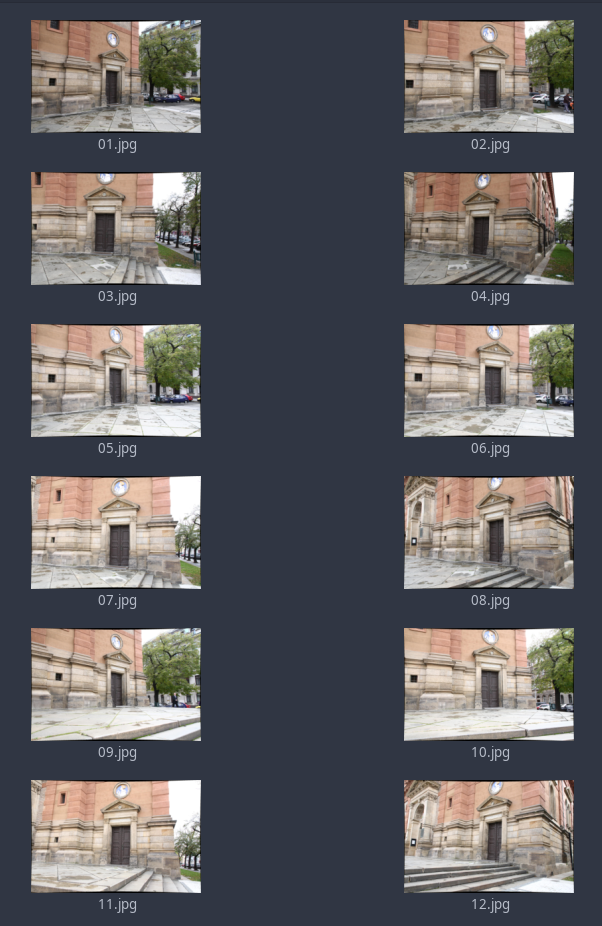
\includegraphics[width=\textwidth]{graphics/input_set.png}
      \caption{Input images.}
      \label{fig:pc_input}
    \end{subfigure}
    \hfill
    \begin{subfigure}[h]{0.65\textwidth}
      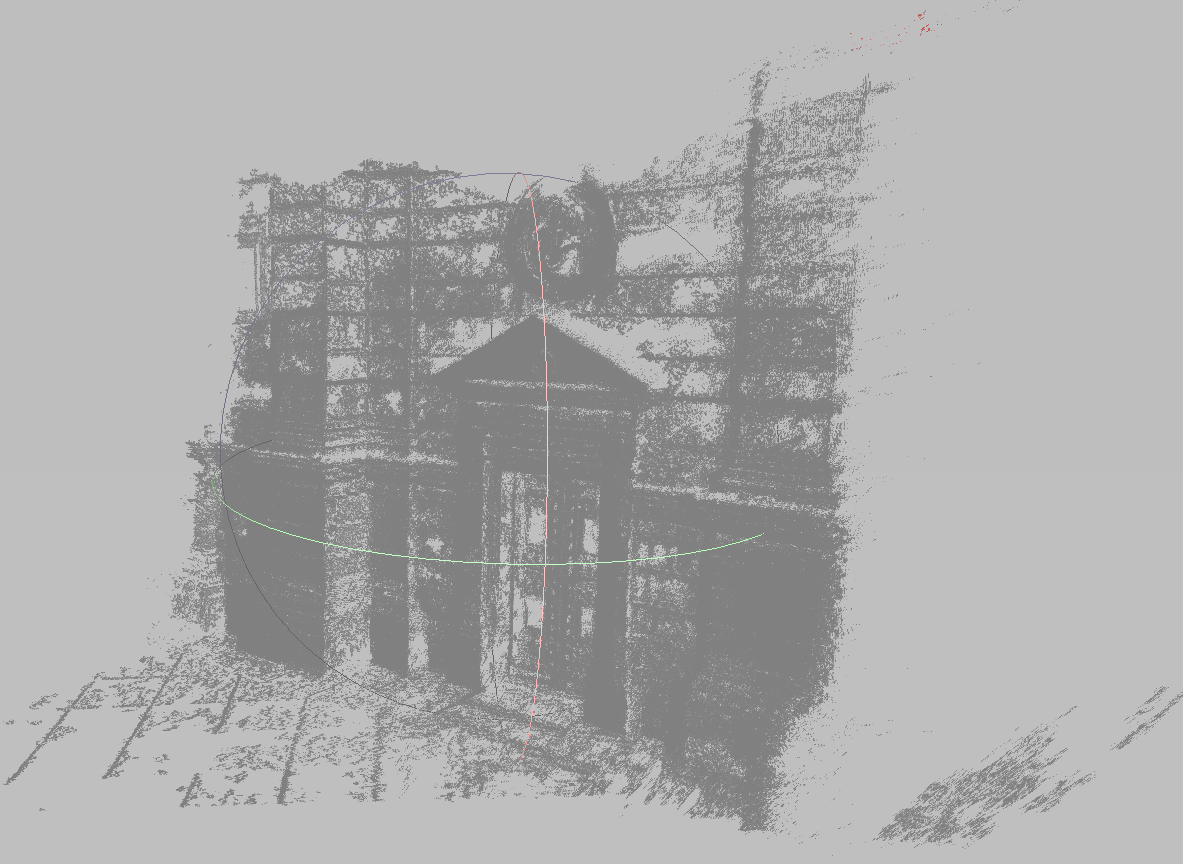
\includegraphics[width=\textwidth]{graphics/reconstructed.png}
      \caption{Output of an SfM algorithm.}
      \label{fig:pc_output}
    \end{subfigure}
    \caption[Ilustration of Structure from Motion.]{Ilustration of Structure from Motion, source - \url{https://github.com/Myralllka/CTU_3d_computer_vision/}}
    \label{fig:pc_recons}
\end{figure}

Structure from Motion (SfM) is another family of algorithms that may be used to implement a system for avoiding obstacles. 
SfM is a method of depth map reconstruction from a continuous sequence of images as in the \autoref{fig:pc_input}.
Using this approach, a dense point cloud as in \autoref{fig:pc_output} can be computed, and obstacles can be detected \cite{Lee2008}. 
This algorithm alone has multiple problems.
Firstly, it can not recover information about such parts of an image as a drone's shadow or any other thing moving with the same velocity in the same direction as a drone.
Secondly, it needs images from at least two timestamps to work.
If there are moving objects, the correct position of them relative to a moving MAV can not be obtained.
Both of these problems can be solved if use SfM with other algorithms.

\section{Problem definition}
\label{sec:problem_definition}
This thesis aims to design a visual obstacle avoidance system for MAVs, create a physical device implementing the system and measure its performance. 
The proposed solution assumes an MAV with a limited size and lifting force that constrains the number, weight and size of its onboard sensory equipment. 
The MAV is thus equipped with two calibrated cameras with a known transformation between them. 
The fields of view of the cameras overlap enough to detect close obstacles.
Framerate of the cameras is sufficient to operate in real-time (at least 30 frames per second (fps)), and the frames are synchronized in time.
The MAV is also equipped with an onboard computer with enough computational power to process the images at a rate sufficient for obstacle avoidance.
The flight environment is assumed to be well-lit and contains objects with well-distinguishable visual features that the cameras can observe.
These features should be unique so that the same feature can be unambiguously matched in images from the two cameras.
The expected output is a reconstruction of the 3D environment around the drone in the form of a set of points representing the nearest objects.
Depending on the estimated distance, these are the possible obstacles that should be avoided.
The system can be integrated with the MAV control system to provide obstacles, so the solution working rate on the MAV's hardware should be sufficient for agile manoeuvering and obstacle avoidance.

